\chapter{IPv6シングルスタックネットワークでのIPv4サービス提供手法}
\label{related}
本章ではIPv6シングルスタックネットワークでのIPv4サービス提供手法を比較し,検討する.


\section{概要}
\label{related:abstract}


第\ref{introduction:background:IPv6-single-stack-network}で述べたように,コンテンツ事業者が運用するIPv6シングルスタックネットワークの重要な役割の一つに,IPv4クライアント端末に対するサービス提供がある.

関連して,アクセスネットワーク網ではIPv6シングルスタックネットワーク上でIPv4によるインターネット接続をクライアントエッジに提供する手法はをIPv4aaS\footnote{IPv4 as a Service}と呼称し,様々な手法が検討されている\cite{RFC8585}.

一方でコンテンツ事業者が運用するネットワークでのIPv4サービス提供においては下のような要件を満たす必要があるため,必ずしもアクセスネットワークでのIPv4aaSと同様の方法が適切であるとは限らない.

\subsection{IPv4サービス提供機構に求められる要件}
\label{related:abstract:requirements}

\subsubsection{IPv4クライアントからのアクセス}
IPv4クライアントに対して透過的にサービスを提供する機構を備える.
一般的なサーバークライアントモデルを想定した場合,インターネット上のIPv4クライアントからサービス提供サーバーに能動的に接続するためには,FQDN\footnote{Fully Qualified Domain Name. 完全就職ドメイン名}もしくはIPv4アドレスをIPv4クライアントが指定出来る必要がある.


\subsubsection{スケーラビリティ}
近年のコンテンツ事業者のネットワークでは,サービスのニーズに合わせて柔軟にスケールアウト\footnote{水平スケール.同等性能の機器を増減させることでサービス容量を拡大・縮小可能なモデル.}可能な設計であることが重要視されている\cite{5550998}.同様にIPv4サービスの提供手法に関しても,事業者のIPv4サービス規模の変化にあわせて柔軟に拡大・縮小可能なアーキテクチャが求められる.

例えば,第\ref{introduction:background:IPv6-single-stack-network:ipv4-service}でも述べたように,将来的にIPv4クライアントの占める割合がIPv6クライアントに相対して低下していった場合に,既設のIPv6ネットワークへの影響を最小限にしつつ,IPv4サービス提供機構を縮小可能であると望ましい.


\subsubsection{IPv4ネットワークへの非依存性}
第\ref{introduction:background:IPv6-single-stack-network}項で述べたように,IPv6シングルスタックネットワークのメリットを最大限に活かすためにはIPv4サービスを提供する場合においてもIPv4ネットワーク及びアドレスに極力依存しないことが望ましい.



\section{IPv4サービス提供手法の分類}
想定されるIPv4サービス提供機構をその技術的差異や狙いを基に以下の3つの手法に分類した.

\subsection{L7リバースプロキシ}

\begin{figure}[h]
    \begin{center}
      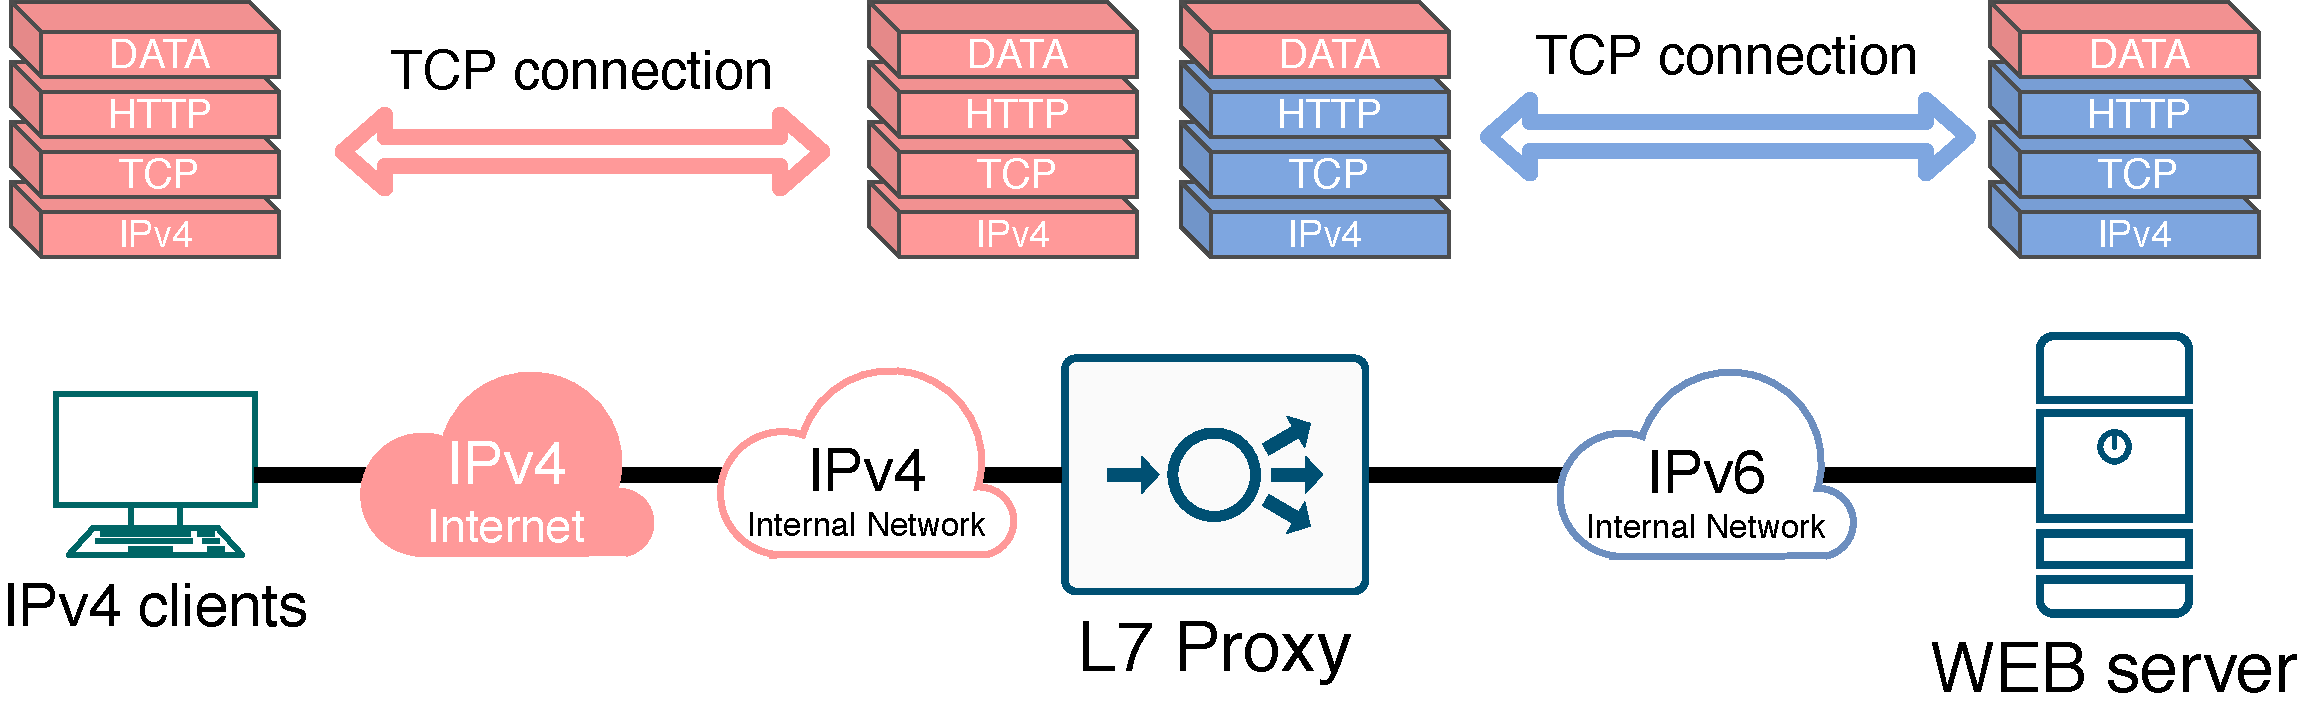
\includegraphics[width=15cm,pagebox=cropbox,clip]{img/L7_proxy_model.pdf}
    \end{center}
    \caption{L7リバースプロキシによるIPv4サービス提供}
    \label{fig:L7_proxy_model}
\end{figure}


L7リバースプロキシとは,クライアントからの接続をプロキシサーバーがアプリケーション層レベルで終端し,プロキシサーバーがクライアントに代わってサーバーと接続する機構である\cite{Gilly2011}.図\ref{fig:L7_proxy_model}に本手法の構成を簡便に示す.主にWEBサーバーへのHTTP接続を負荷分散するための手法として広く採用されている.

IPv6シングルスタックネットワークにおいてIPv4サービスを提供するためには,IPv4インターネットとの接続点からプロキシサーバーまでの間にIPv4ネットワークを配備する必要がある.

IPv4・IPv6間のプロトコル仕様の差を考慮する必要が無いため互換性に留意する必要が無い点や,MTU\footnote{Maximum Transmission Unit.ここでは一つのパケットに搭載可能なデータ量を指す.}を減らさずにアプリケーショントラフィックを伝送可能である点が利点に挙げられる.

一方でアプリケーションレイヤーでのコネクション終端やそのステート管理を行う必要があるため,プロキシサーバーに負荷が掛かるため高性能な機器の導入が必要になる.

またスケールアウトを可能にするためにL4LBと組み合わせた3ステージのアーキテクチャ利用する手法が近年主流である\cite{Facebook_LB, Google_LB}が,この手法を採用するためには,ある程度のIPv4ネットワークを配備する必要があり,第\ref{related:abstract:requirements}項で述べた要件に合致せず,IPv6シングルスタックネットワークのメリットを損なうことになる.



\subsection{IPv4/IPv6トンネリング}
\begin{figure}[h]
    \begin{center}
      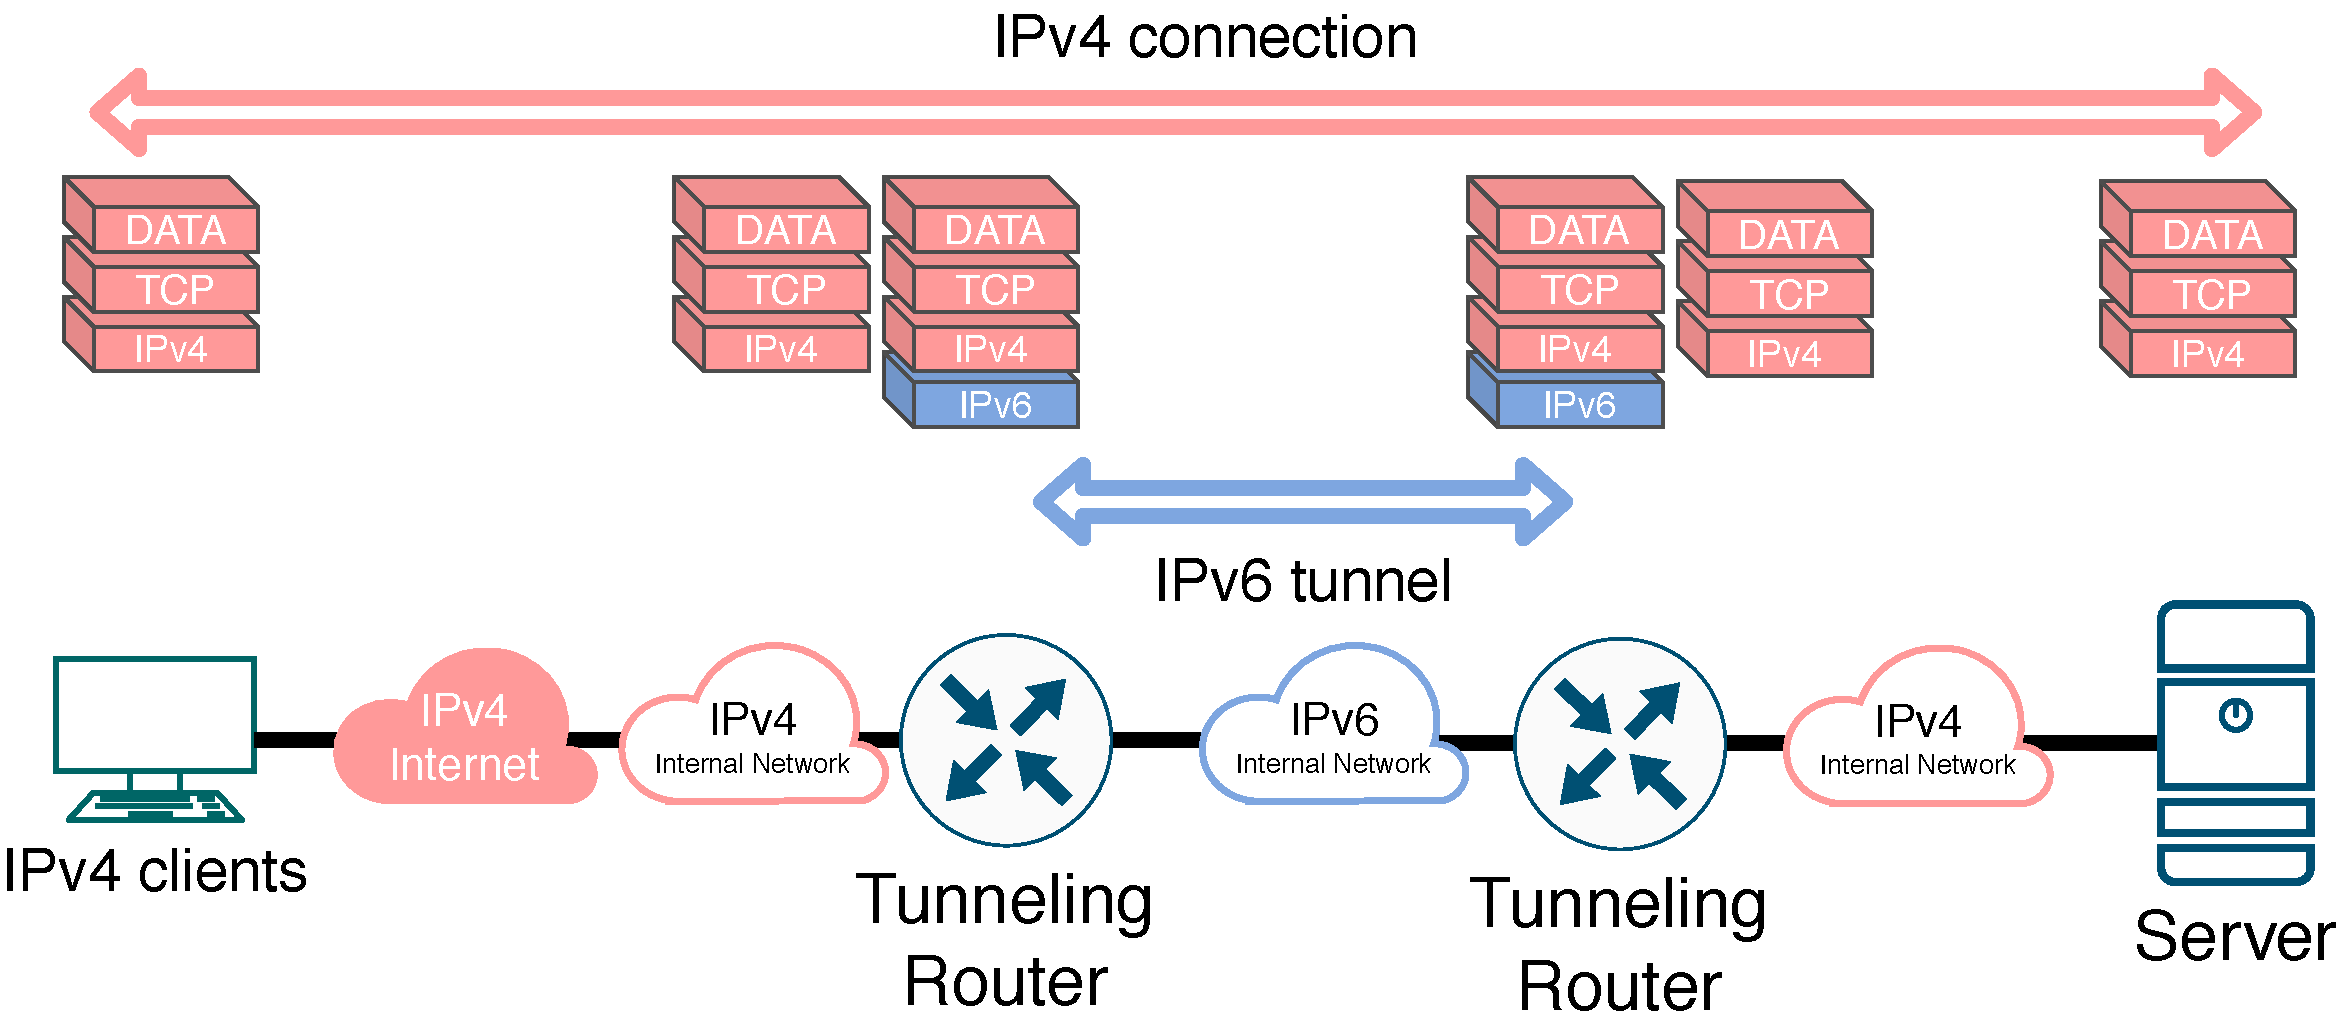
\includegraphics[width=15cm,pagebox=cropbox,clip]{img/Tunneling_model.pdf}
    \end{center}
    \caption{IPv4/IPv6トンネリングによるIPv4サービス提供}
    \label{fig:tunneling_model}
\end{figure}

IPv4/IPv6トンネリングとは,IPv4パケットをIPv6パケットによってカプセリングすることでIPv6ネットワークを通過させる手法である.IPv4トラフィックを透過的に利用することが出来るため,アクセスネットワークで最も一般的に利用されているIPv4aaS手法である\cite{RFC8585}.図\ref{fig:tunneling_model}に本提供手法の構成を簡便に示す.

IPv6シングルスタックにおけるIPv4サービス提供手法としては,IPv4クライアントから到達したパケットをトンネルルーターによって一度IPv6パケットでカプセリングし,IDC内のIPv6シングルスタックネットワークを通過させ,IPv4サービス提供サーバー上もしくはその直前で再びでカプセリングを解くことで,IPv4提供サーバーまでネイティブなIPv4トラフィックを通過させる運用が考えらえる.
IPv4ネットワークをサーバーで利用できるため,多種多様なアプリケーションでの採用が期待できる.

しかしながら,トンネルルーターとIPv4サービスサーバー間にある程度のIPv4ネットワークを配備しなければならず,ToR\footnote{Top of rack switch. ここではサーバーのL2終端を行うルーターを指す.}及びサーバーではIPv4/IPV6デュアルスタック運用が必要になるため,第\ref{related:abstract:requirements}項で上げた要件である「IPv4ネットワークへの非依存性」に合致しない.また,トンネルプロトコルの多く\cite{6799698}はは基本的に1:1もしくは1:Nの接続が基本となるため,水平スケールさせることが困難である.



\subsection{IPv4/IPv6トランスレーション}
\begin{figure}[h]
    \begin{center}
      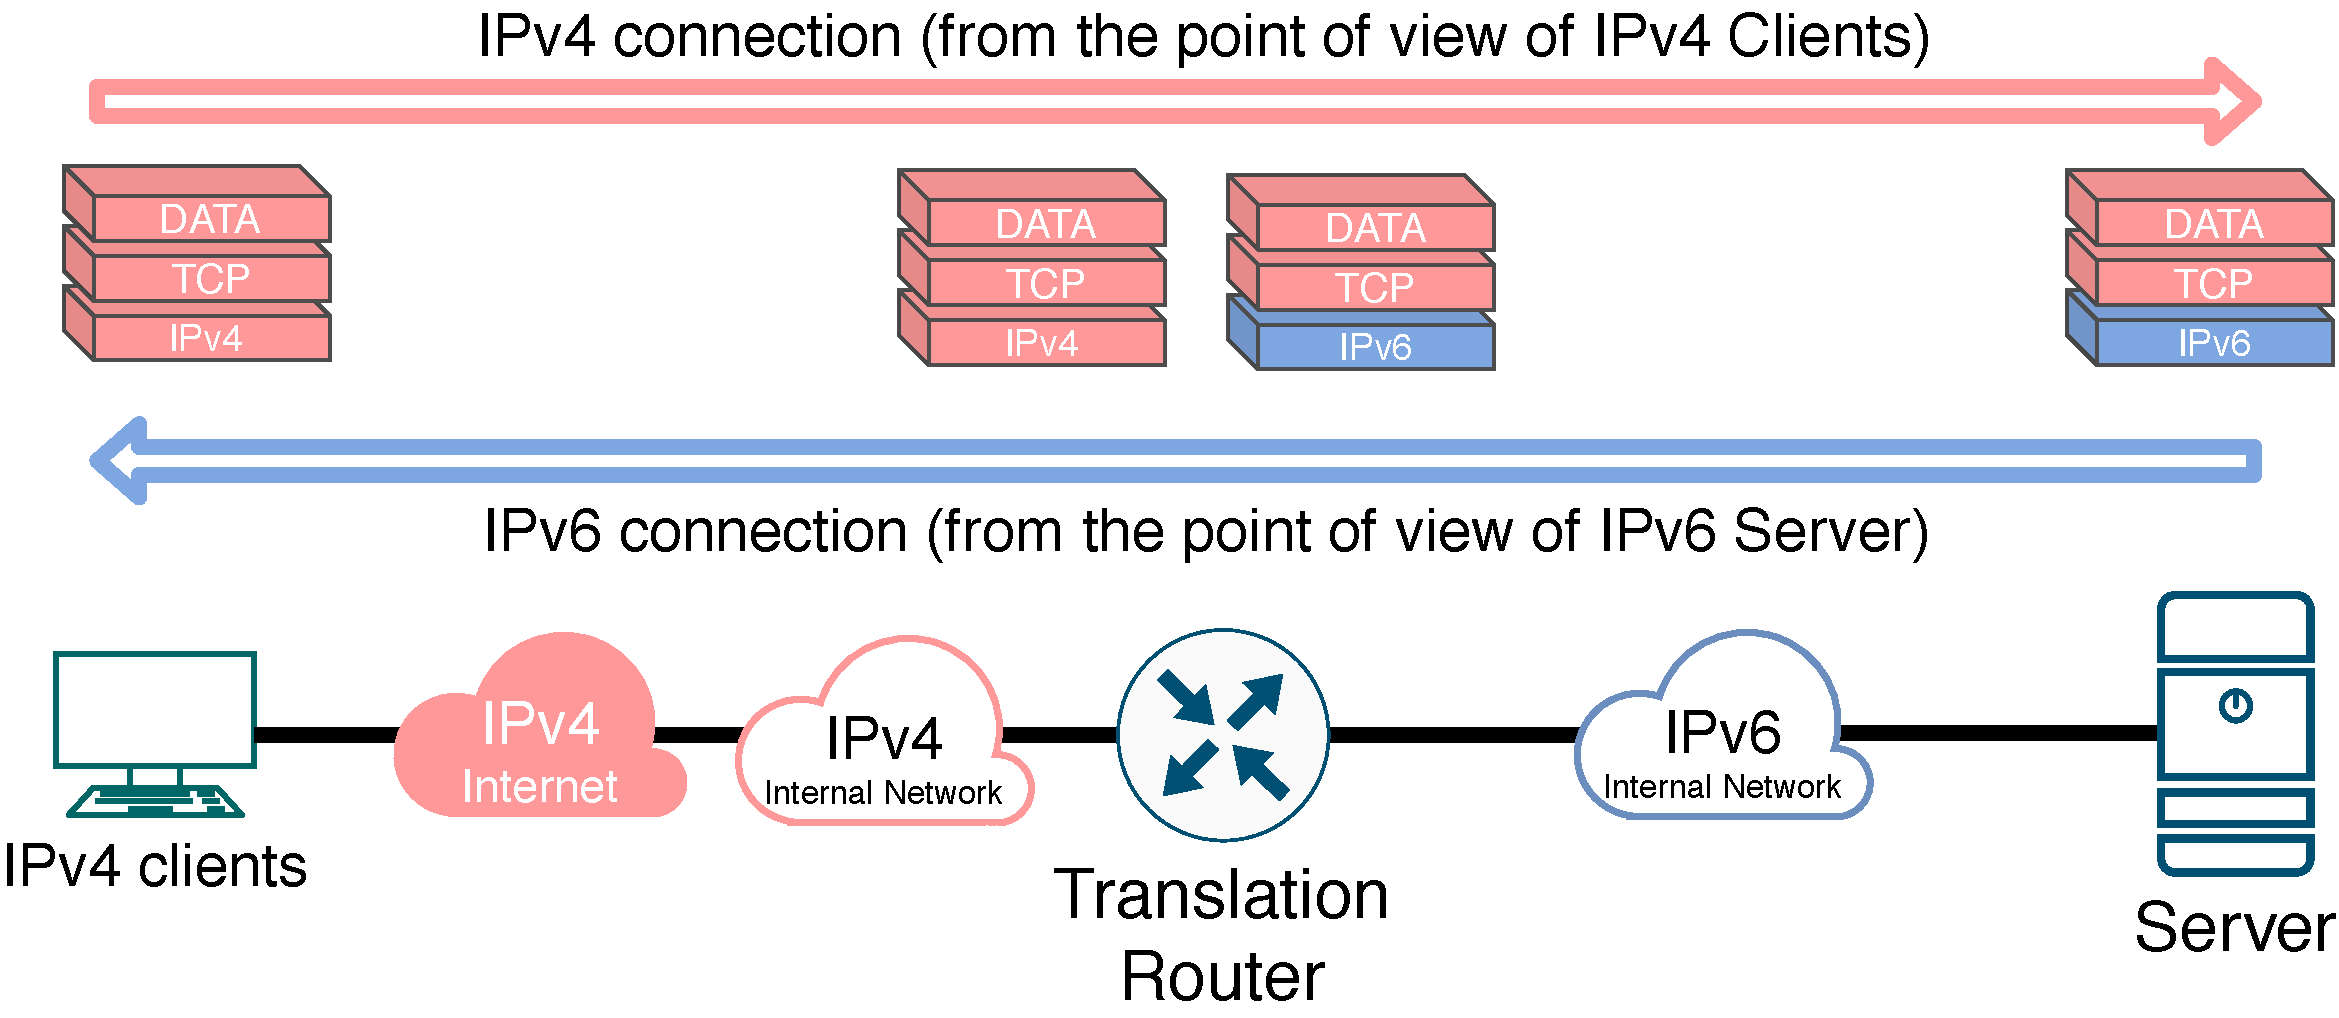
\includegraphics[width=15cm,pagebox=cropbox,clip]{img/translation_model.pdf}
    \end{center}
    \caption{IPv4/IPv6トランスレーションによるIPv4サービス提供}
    \label{fig:tunneling_model}
\end{figure}

IPv4/IPv6トランスレーションとは,IPv4パケットとIPv6パケットをIP/ICMP変換アルゴリズム\cite{RFC7915}を利用して相互に変換する手法である.$1:N$の関係でアドレス・ポート変換を行うステートフルモードと,$1:1$でアドレス変換を行うステートレスモードが定義されている.IPv4ネットワークとIPv6ネットワークの境界に位置する変換ルーターにより,相互にプロトコル変換が行われる.

IPv4/IPv6トランスレーションではIPv4アドレスをIPv6アドレスとして表現することが要求されるが,変換プレフィックスと呼ばれるIPv6ネットワークプレフィックスにIPv4アドレスを埋め込むことで,任意のIPv4アドレスをIPv6ホストから認識可能な形で表現する.変換プレフィックスにはRFC6052で定義された64:ff9b::/96の他に,運用者が専有可能なGUA\footnote{Global Unicast Address. }の/96のIPv6プレフィックスを利用することが想定されている\cite{RFC6052}.

図\ref{fig:tunneling_model}で示すように,変換ルーター以外のホストがIPv4ネットワークに属する必要が無いため,第\ref{related:abstract:requirements}項で述べた「IPv4ネットワークへの非依存性」の面で,他の2手法より優れていると言える.また,IPv4サービスを行うサーバーから変換ルーターの間はネイティブなIPv6ネットワークで接続可能なため,ECMP\cite{rfc2992}による経路の冗長化が可能なほか,ステートレスモードでは変換ルーターの水平スケールが可能な点で,IPv6シングルスタックネットワークにおけるIPv4サービス提供に求められる要件を満たしやすい.


一方でIPv4とIPv6のプロトコル実装に差があるため,コンテンツ事業者のサービスの内容によってはサービス影響を考慮する必要がある点は留意すべきである.

